\documentclass[10pt]{beamer}

\usetheme{metropolis}
\usepackage{appendixnumberbeamer}


\usepackage{booktabs}
\usepackage[scale=2]{ccicons}

\usepackage{pgfplots}
\usepgfplotslibrary{dateplot}

\usepackage{xspace}
\newcommand{\themename}{\textbf{\textsc{metropolis}}\xspace}

\usepackage{graphicx}
\usepackage{animate}

\usepackage{tikz}
\usetikzlibrary{arrows,shapes}

\tikzstyle{every picture}+=[remember picture]
\tikzstyle{na} = [baseline=-.5ex]

\usepackage{amsmath, mathtools, bm}

\usepackage{hyperref}

\title{Issues in earthquake modelling}
\subtitle{}
\date{3$^{\text{rd}}$ September 2019 }
\author{Zak Varty$^1$ \\ J. Tawn$^1$, P. Atkinson$^1$, S. Bierman$^1$ }
 \institute{$^1$Lancaster University, $^2$Shell Global Solutions}
%  \titlegraphic{\hfill\includegraphics[height=1.5cm]{logo.pdf}}

\begin{document}

\begin{frame}{\ }
 \begin{center}
    \hline
      \textbf{Issues in earthquake modelling} \\
      \vspace{0.3cm}
     Zak Varty$^1$, Jonathan Tawn$^1$, Peter Atkinson$^1$ \& Stijn Bierman$^2$ \\
     $^1$Lancaster University, UK. \quad $^2$Shell Global Solutions, NL.
    \hline
    \tikz [remember picture,overlay]
    \node[opacity=0.6] at
        ([yshift=-4.2cm,xshift= -5.9cm]current page.center) 
        %or: (current page.center)
        {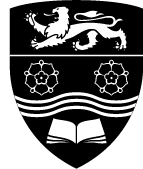
\includegraphics[width=0.07\textwidth]{Images/lancaster_black1.png}};
 \end{center}
 \vfill 
    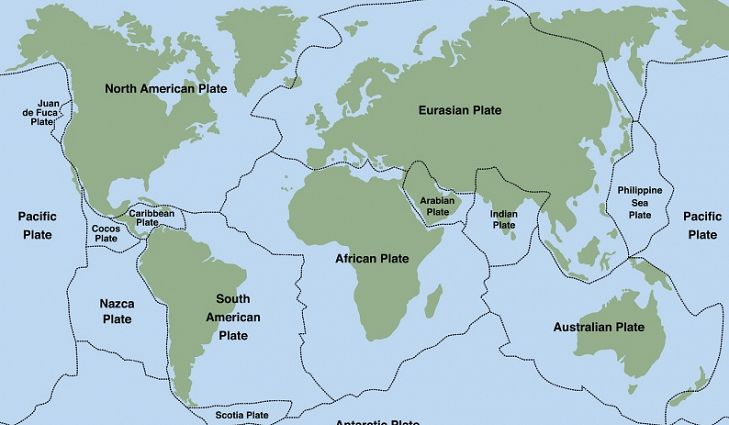
\includegraphics[height = 2.8cm]{Images/tectonic-plates.jpg}
    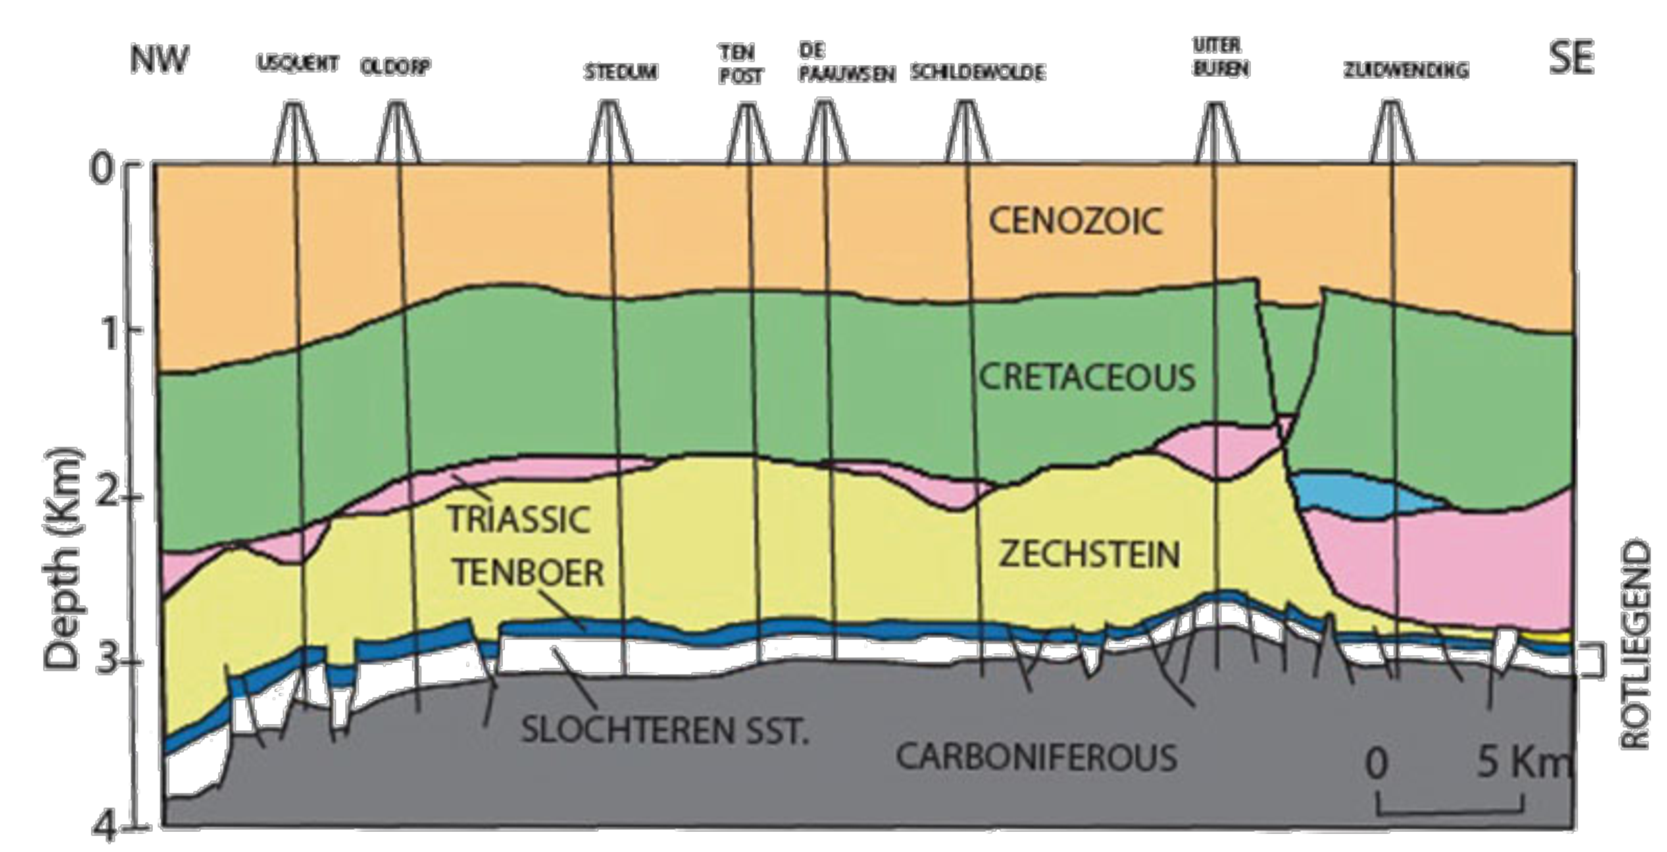
\includegraphics[height = 2.8cm ]{Images/layers.pdf}
    \vfill
\end{frame}

\begin{frame}{ \hfill What do we want to do?}
\begin{columns}
\begin{column}{0.5\textwidth}
   \begin{itemize}
   \vfill
        \item Link gas extraction and earthquakes above the magnitude of completion.
    \vspace{0.3cm}
        \item Investigate the possibility of aftershocks and their properties. 
    \vspace{0.3cm}
        \item Use the resulting model to forecast under different extraction scenarios. 
    \vfill
    \end{itemize}
\end{column}
\begin{column}{0.5\textwidth}  %%<--- here
    \begin{center}
     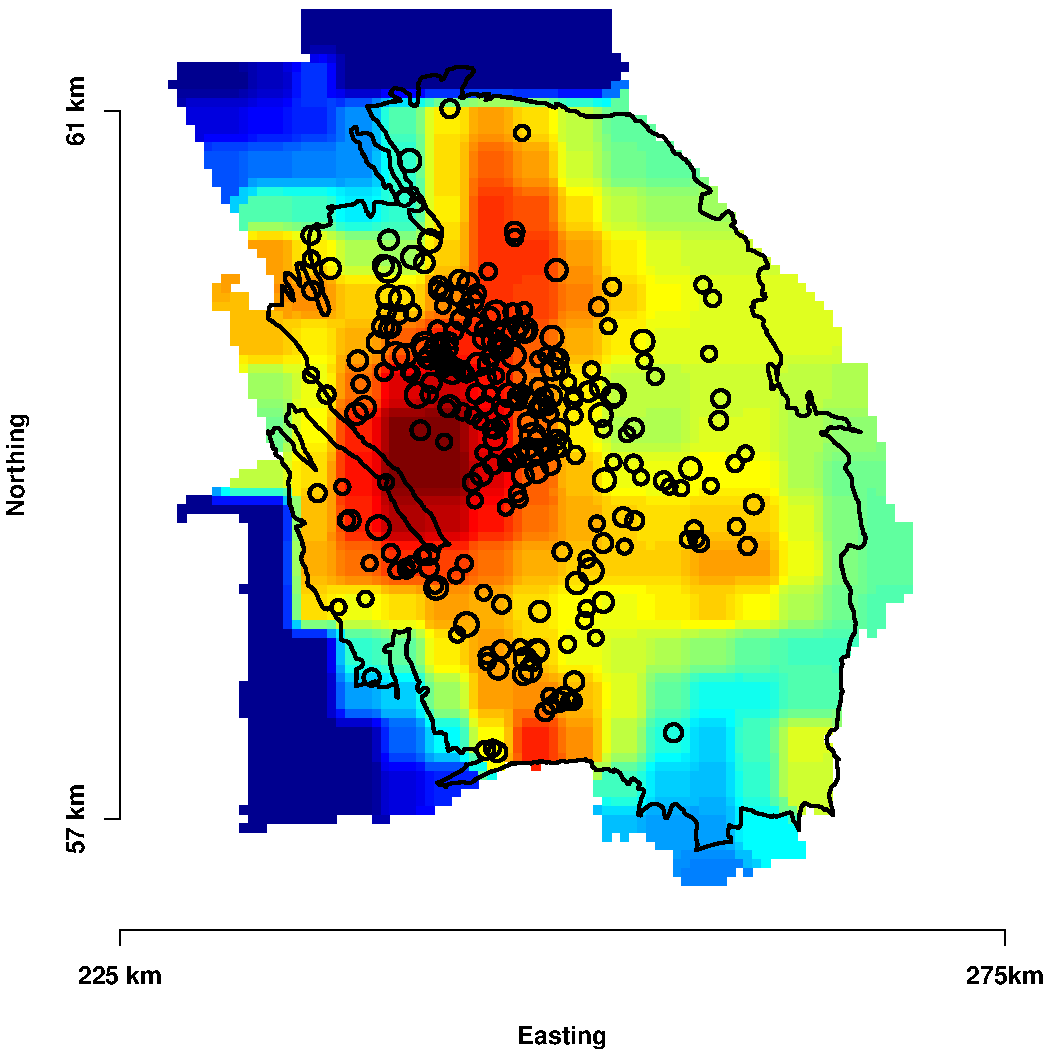
\includegraphics[width=\textwidth]{Images/Cumulative_Compaction+Event_ContoursII.pdf}
     \end{center}
\end{column}
\end{columns}
    \tikz [remember picture,overlay]
    \node[opacity=0.6] at
        ([yshift=-4.2cm,xshift= -5.9cm]current page.center) 
        %or: (current page.center)
        {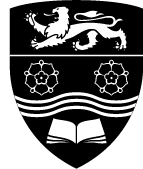
\includegraphics[width=0.07\textwidth]{Images/lancaster_black1.png}};
\end{frame}


\begin{frame}{\hfill Current approach}
\begin{columns}
\begin{column}{0.35\textwidth}
   \begin{itemize}
   \vfill
     \item Model earthquakes as a marked, self exciting point process.
    \vspace{0.3cm}
     \item \textbf{Issue:} Highly correlated parameters from using empirical earthquake `laws'.
    \vfill
    \end{itemize}
\end{column}
\begin{column}{0.65\textwidth}  %%<--- here
     \begin{equation*}
    \footnotesize{
         \begin{array}{rcc}
         &&   \overbracket{\mu(\bm{x},t | X, \theta)}^{\text{Poisson mainshocks}}   \\
          \underbracket{\lambda(\bm{x},t| X, \mathcal{H}_t, \theta)}_{\text{All earthquakes}} & \ =  &  + \\
           && \underbracket{\sum_{i:t_i<t}\kappa(m_i|\theta)g(t-t_i|\theta)h(\bm{x}-\bm{x}_i|\theta)}_{\text{ETAS aftershocks}}.
        \end{array}
    }
    \end{equation*}
    \centering
    \vspace{0.5cm}
    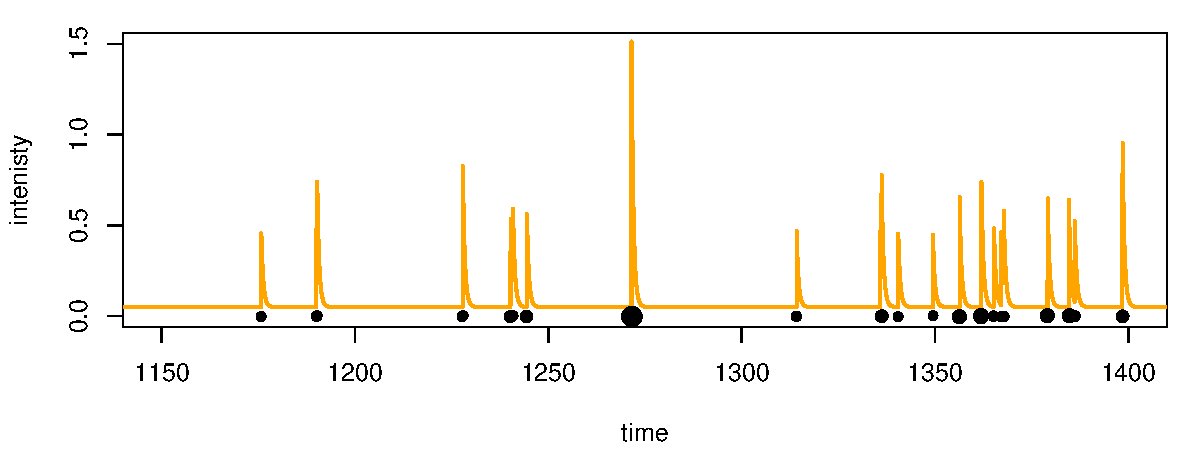
\includegraphics[width = \textwidth]{Images/ETAS_intensity.pdf}
    
\end{column}
\end{columns}
    \tikz [remember picture,overlay]
    \node[opacity=0.6] at
        ([yshift=-4.2cm,xshift= -5.9cm]current page.center) 
        %or: (current page.center)
        {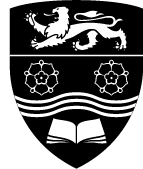
\includegraphics[width=0.07\textwidth]{Images/lancaster_black1.png}};
\end{frame}



\begin{frame}{\hfill Improvements from extreme value theory}
    \begin{itemize}
        \item We want flexible tail models for $g(t)$ and $h(\bm{x})$ and for magnitudes above a threshold: EVT a natural resource. 
        \item Centre the productivity effect $\kappa(m)$ about mean magnitude.
    \end{itemize}
   \begin{columns}
    \begin{column}{0.33\textwidth}
    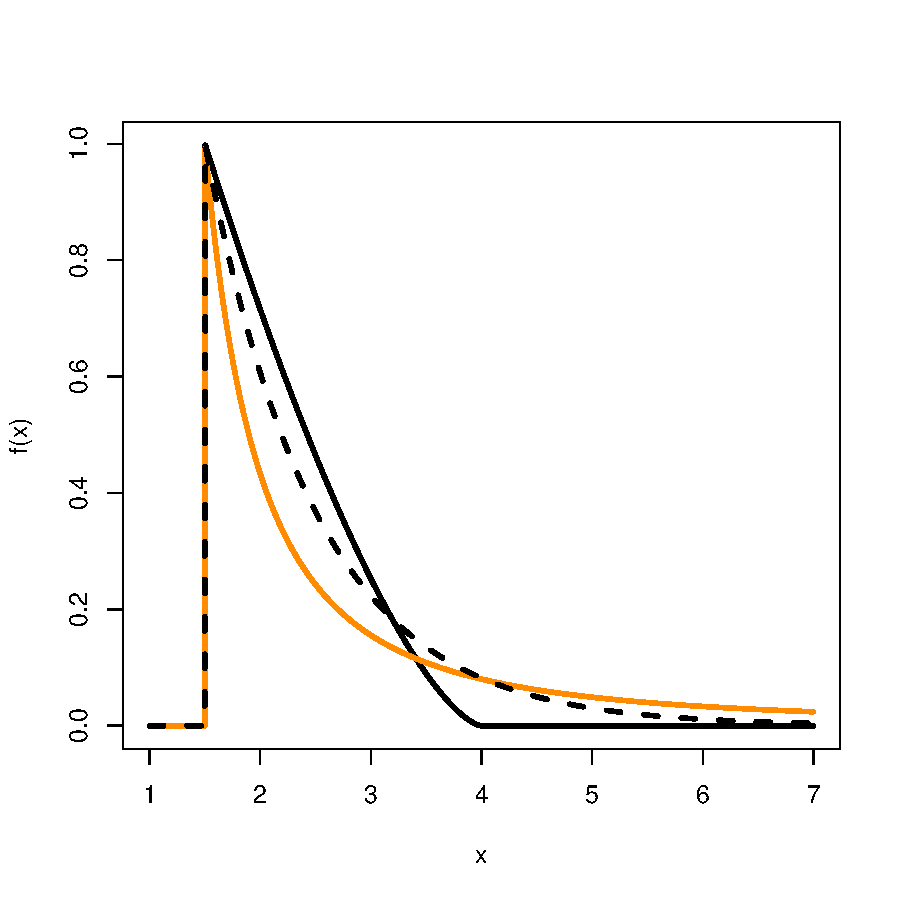
\includegraphics[width = \textwidth]{Images/GPD_examples.pdf}
    \end{column}
    \begin{column}{0.33\textwidth}
    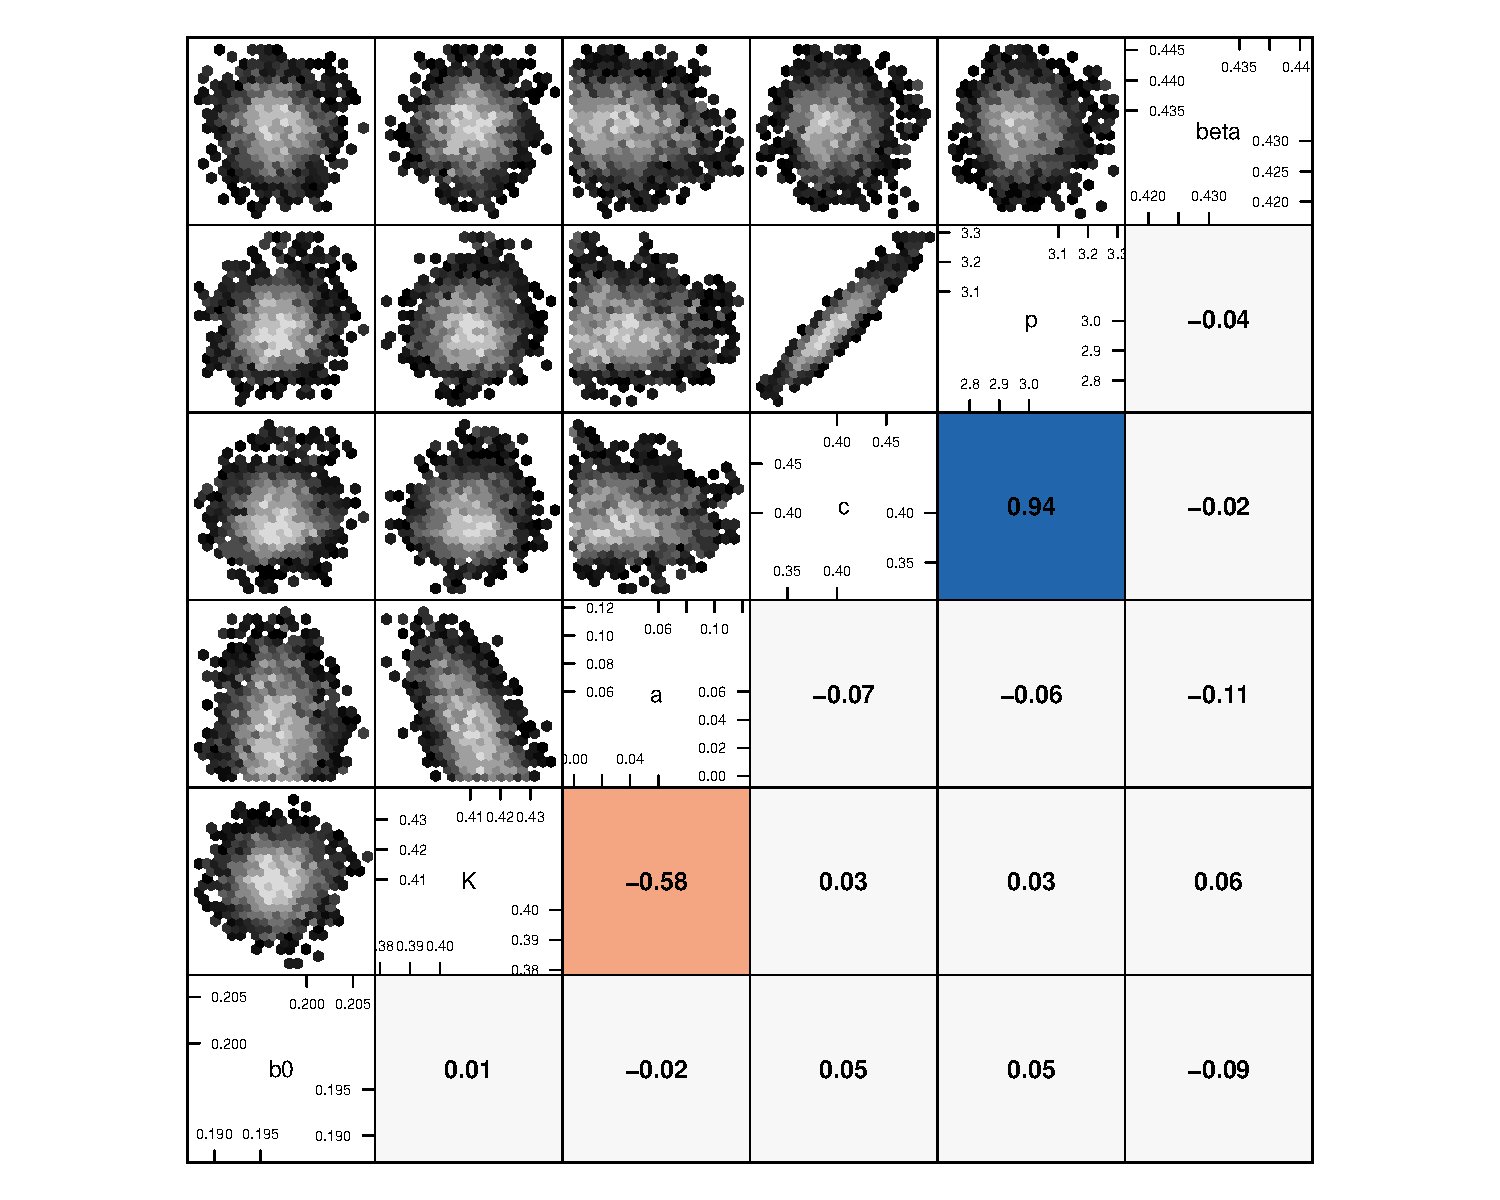
\includegraphics[width = \textwidth]{Images/ETASpars.pdf}
    \end{column}
    \begin{column}{0.33\textwidth}
    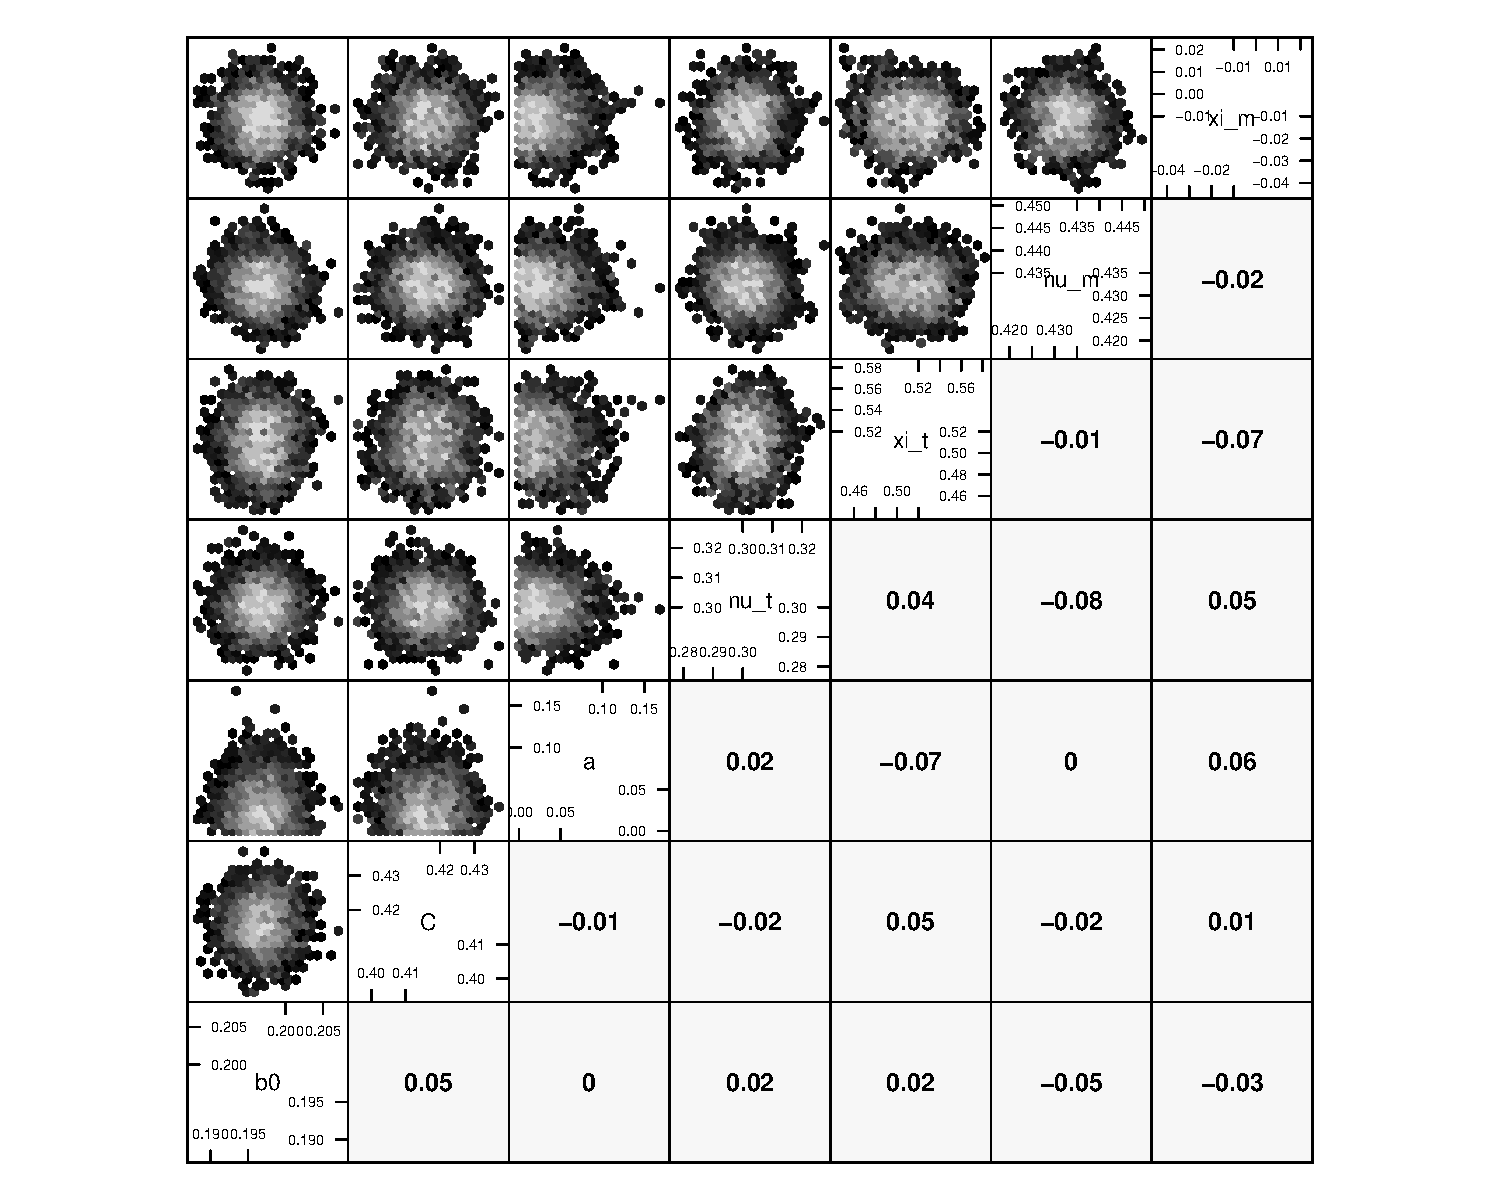
\includegraphics[width = \textwidth]{Images/cGPDpars.pdf}
    \end{column}
    \end{columns}
    
    \begin{itemize}
         \item Model made more flexible and parameter dependence reduced.
    \end{itemize}
        \tikz [remember picture,overlay]
    \node[opacity=0.6] at
        ([yshift=-4.2cm,xshift= -5.9cm]current page.center) 
        %or: (current page.center)
        {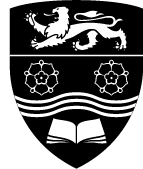
\includegraphics[width=0.07\textwidth]{Images/lancaster_black1.png}};
\end{frame}

\begin{frame}{\hfill Can you help?}
    \begin{itemize}
    \vfill
        \item Many open statistical problems in induced seismicity.
        \vfill
        \item The current approach benefits from using ideas in EVT.  
        \vfill
        \item How about other areas: \\Epidemiology, survival analysis, finance, ecology?
        \vfill
        \item Completely different approach inspired by your area? \\ Any ideas very welcome!
        \vfill
    \end{itemize}
    \textbf{ Twitter:} @zakvarty \hfill \textbf{Email:} z.varty@lancs.ac.uk 
    
        \tikz [remember picture,overlay]
    \node[opacity=0.6] at
        ([yshift=-4.2cm,xshift= -5.9cm]current page.center) 
        %or: (current page.center)
        {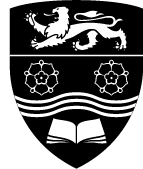
\includegraphics[width=0.07\textwidth]{Images/lancaster_black1.png}};
\end{frame}

\end{document}
